\documentclass{beamer}
\usepackage[OT1]{fontenc}
\usepackage[utf8]{inputenc}
%\setmainfont{STIX}
%\usepackage{unicode-math}
%\setmathfont{STIX Math}

\usepackage[british]{babel}

\usepackage[export]{adjustbox}

%\usepackage{cite}
\usepackage{graphicx}
\usepackage{amsmath}
\usepackage{caption}

\usepackage{multirow}

\usepackage{mathtools}
\usepackage{bm}
\usepackage{textcomp}
\let\v\bm
\def\mat#1{\bm{#1}}
\def\mul{\cdot}

\usepackage{siunitx}

\usepackage[linesnumbered,ruled]{algorithm2e}
\newcommand{\KwAssign}{\ensuremath{\leftarrow}}

\usepackage{url}

\title{Biotech Beer Brewing}
\subtitle{Or: How I Learned to Stop Worrying and Control the Lactobacilli}
\author{Dominik Schmidt, ETH Zürich\\Jakob Wittman, TU München}
\institute{Háskóli Íslands}
\date{\today}
\titlegraphic{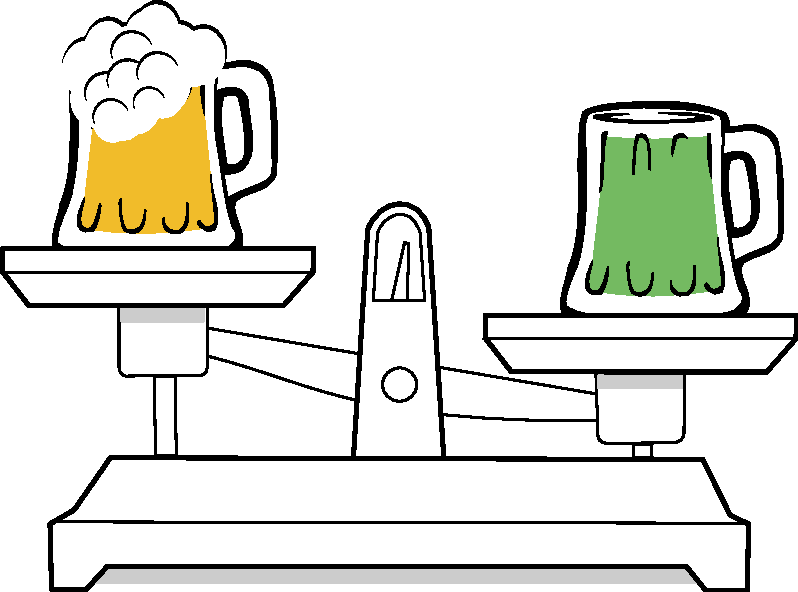
\includegraphics[width=0.3\linewidth]{../Graph/Logo.pdf}}
\logo{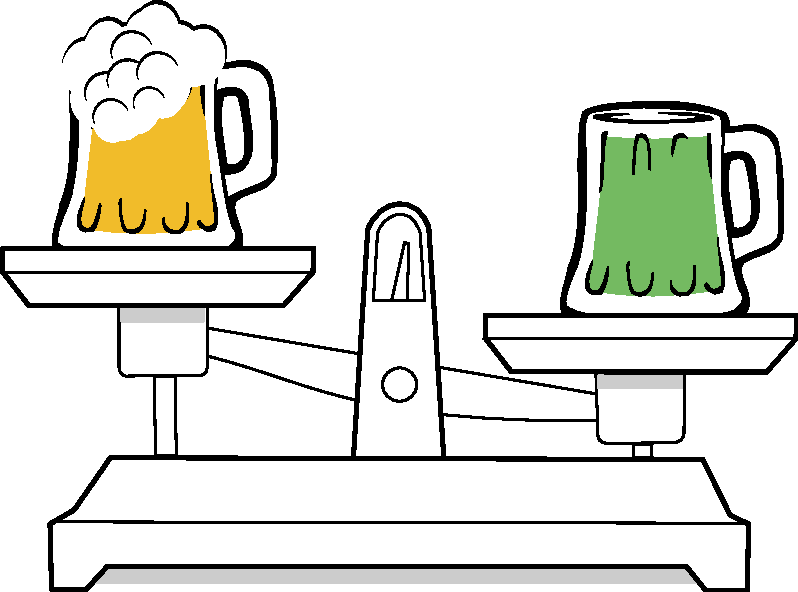
\includegraphics[width=5em]{../Graph/Logo.pdf}}
\beamertemplatenavigationsymbolsempty

\usepackage{xcolor}
\usepackage{tikz}
\usetikzlibrary{calc}
\usetikzlibrary{arrows}
\usetikzlibrary{positioning}

\begin{document}
\begin{frame}[plain]
	\titlepage
\end{frame}
\begin{frame}
  \frametitle{Content}
  \tableofcontents
\end{frame}

\section{Introduction}
\begin{frame}{Introduction}
  \begin{block}{Contamination in alcoholic fermentation}
    \begin{itemize}
      \item Bacterial contamination lowers the productivity of yeast (up to 30\% loss)
      \item mostly Lactobacillus plantarum and wild yeasts
      \item high quality standards in food industry (beer, wine, whisky,...)
    \end{itemize}
  \end{block}

  \begin{block}{How find process optimizations?}
    \begin{itemize}
     \item experiments with real cultures are expensive and time consuming
     \item simulation methods using genome-scale models gaining popularity
    \end{itemize}
  \end{block}
\end{frame}

\begin{frame}{Material}{Overview}

\begin{figure}[!h]
%\centering
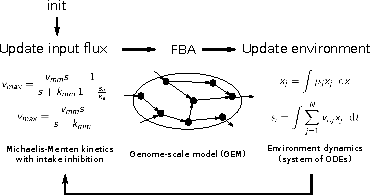
\includegraphics[width=\linewidth]{Img/dfba.pdf}
\caption{Dynamic flux balance analysis iteration step}
\label{fig:dfba}
\end{figure}

% \begin{equation} \label{eq:diff_eq_x}
%  x_j = \int \mu_j x_j \;\; \mathrm{d}x
% \end{equation}
% \begin{equation} \label{eq:diff_eq_s}
%  s_i = \int \displaystyle\sum_{j=1}^{N} v_{i,j} x_j  \;\; \mathrm{d}t
% \end{equation}
% 
% \begin{equation} \label{eq:michaelis-menten}
%  v_{max} = \frac{v_{mm} s}{s + k_{mm}} \frac{1}{1 + \frac{s_a}{k_{a}}}
% \end{equation}
% \begin{equation} \label{eq:michaelis-menten}
%  v_{max} = \frac{v_{mm} s}{s + k_{mm}}
% \end{equation}
  
\end{frame}

\section{Material}
\begin{frame}{Material}{Tools}
%   \begin{block}{Building blocks}
%     \begin{itemize}
%       \item Genome-scale models (GEM) to simulate bacteria behavior
%       \item Flux balance analysis (FBA)
%       \item Environment dynamics modeled in system of ordinary differential equations
%       \item Metabolite kinetics models using Michaelis-Menten constants
%     \end{itemize}
%   \end{block}
  
%   \begin{block}
    \begin{itemize}
      \item python 3
      \item dopri5 ODE solver, scipy.integrate.ode package \cite{hairer1993solving}
      \item COBRApy package \cite{heirendt_creation_nodate}
      \item \textit{Dynamic Multispecies Metabolic Modeling} (DMMM) framework (Matlab)\cite{zhuang_design_2012}
    \end{itemize}
% 
%   \end{block}


  
\end{frame}

\section{Material}
\begin{frame}{Material}{Simulation setup}
  
\end{frame}

\section{Results}
\begin{frame}
  
\end{frame}

\section{Conclusions and next steps}
\begin{frame}
  
\end{frame}

\appendix
\section<presentation>*{\appendixname}
\subsection<presentation>*{For Further Reading}
\begin{frame}[allowframebreaks]
  \frametitle{References}
  
  \bibliographystyle{IEEEtran}
  \bibliography{./../final_report/references.bib}
  
  
%   \begin{thebibliography}{10}
%     
%   \beamertemplatebookbibitems
%   % Start with overview books.
% 
%   \bibitem{Author1990}
%     A.~Author.
%     \newblock {\em Handbook of Everything}.
%     \newblock Some Press, 1990.
%  
%     
%   \beamertemplatearticlebibitems
%   % Followed by interesting articles. Keep the list short. 
% 
%   \bibitem{Someone2000}
%     S.~Someone.
%     \newblock On this and that.
%     \newblock {\em Journal of This and That}, 2(1):50--100,
%     2000.
%   \end{thebibliography}
\end{frame}


% \section{What}
% 	\begin{frame}{What?!}
% 		\begin{minipage}{0.45\linewidth}
% 		\begin{itemize}
% 			\item Analyse coexistance of:
% 			\begin{itemize}
% 				\item Saccharomyces cerevisiae
% 				\item Lactobacillus plantarum
% 			\end{itemize}
% 			\item Understand how beer can turn sour
% 			\item See how sour beer can be prevented
% 		\end{itemize}
% 		\end{minipage}
% 		\begin{minipage}{0.45\linewidth}
% 		\centering
% 		\begin{tikzpicture}
% 			\node[left] at(0, 6) (yeast){Yeast};
% 			\node[right] at(2, 6) (la){Lactobacilli};
% 			\node[above] at(1, 6.5) (ox){$\mathsf{O_2}$};
% 			\fill[fill=yellow] (0,0) -- (0,3) -- (2,3) -- (2,0) arc(0:-180:1 and 0.5);
% 			\draw (0,0) -- (0,5) arc(180:0:1 and 0.5) -- (2,0) arc(0:-180:1 and 0.5);
% 			\draw[-latex] (yeast.east) .. controls +(right:0.5) and +(up:0.5) .. (0.75,5);
% 			\draw[-latex, dashed] (la.west) .. controls +(left:0.5) and +(up:0.5) .. (1.25,5);
% 			\draw[-|] (ox.south) -- (1,6);
% 		\end{tikzpicture}
% 		\end{minipage}
% 	\end{frame}
% \section{How}
% 	\begin{frame}{How?}
% 		\begin{itemize}
% 			\item Find beer-like initial conditions of medium
% 			\item Metabolite density via intake upper bounds
% 			\item Simulate population dynamics via $\mathsf{V_{Bio}}$
% 			\item Simluate metabolite flow and update the medium concentrations
% 			\item Homogeneity of medium is assumed
% 		\end{itemize}
% 		\begin{center}
% 		\begin{tikzpicture}[x=0.1\linewidth,y=0.1\linewidth]
% 			\tikzset{box/.style={shape=rectangle, draw=black,align=center}}
% 			\tikzset{flow/.style={-latex}}
% 			\node[box] (medium){Update\\Medium};
% 			\node[box, right=of medium] (bounds){Adapt\\Models};
% 			\node[box, right=of bounds](opt){Optimize\\$\mathsf{V_{Bio}}$};
% 			\node[box, right=of opt](sim){\tikz[scale=0.5]{\draw[<->](0,3) -- (0,0) -- (5,0); \draw[red] (0,2) .. controls (0.5,2) and (2,2) .. (3,3);\draw[green] (0,1) .. controls (0.5,0.5) and (2,0.25) .. (3,0.25); \draw[dashed] (3,3) -- (3,0) node[below]{$\Delta t$};}};
% 			\draw[flow] (medium.east) -- (bounds.west);
% 			\draw[flow] (bounds.east) -- (opt.west);
% 			\draw[flow] (opt.east) -- (sim.west);
% 			\draw[flow] (sim.south) -- +(down:0.5) -| (medium.south);
% 		\end{tikzpicture}
% 		\end{center}
% 	\end{frame}
% \section{Why}
% 	\begin{frame}{Why}
% 		\begin{itemize}
% 			\item Find conditions favourable for good beer
% 			\item Level up our brewing skills 
% 			\item Help small-scale and craft breweries
% 			\item Potentially reduce desinfectant use in the industry
% 		\end{itemize}
% 		\begin{figure}
% 			\centering
% 			
\includegraphics[width=0.3\linewidth]{Img/AMIV_Braeu.pdf}
% 		\end{figure}
% 	\end{frame}
\end{document}
